\documentclass[11pt,a4paper]{report}
%\usepackage[utf8]{inputenc}
\usepackage[latin1]{inputenc}
\usepackage{amsmath}
\usepackage{amsfonts}
\usepackage{amssymb}
\usepackage{multicol, blindtext}
\usepackage[top=0.58in, bottom=0.9in]{geometry}
\usepackage{textcomp}
\usepackage{graphicx}
\usepackage{lipsum}

\title{	\begin{figure}[h]
			\centering
			
\includegraphics[scale=0.75]{./pictures/logoufpa.png}
			\label{fig:logoufpa}
		\end{figure}
		Universidade Federal do Par� \linebreak
		Instituto de Tecnologia \linebreak
		Faculdade de Engenharia de Computa��o e Telecomunica��es \linebreak
		Sistemas de Controle \linebreak
		Experi�ncia 4 (Projeto por aloca��o de p�los) com $MatLab^{\copyright}$ \linebreak
		Prof$^{a}$ Adriana Castro}

\begin{document}

\author{Danilo Souza - 10080000801}
\maketitle

\tableofcontents
\listoffigures

\chapter{Experimento 1}

	As Figuras \ref{fig:experimento1_LGR_original}, \ref{fig:experimento1_LGR_zero} e \ref{fig:experimento1_LGR_polo} mostram, respectivamente, o LGR de $G(s) = \frac{2}{s(s+1)}$, o LGR de $G(s) = \frac{2(s+2)}{s(s+1)}$e o LGR de $G(s) = \frac{2}{s(s+1)(s+2)}$. Quando um zero � adiconado ao LGR, o sistema permanece est�vel para qualquer valor positivo de $K$ ($K \geqslant 0$). Quando um p�lo � adicionado ao LRG, conforme o servado abaixo, o LGR entra para o plano da instalbilidade (SPD), fazendo com que o valor de K possua uma faixa limitada de estabilidade que neste caso � $K \leqslant 3$.
	
		\begin{figure}[h!]
			\centering
			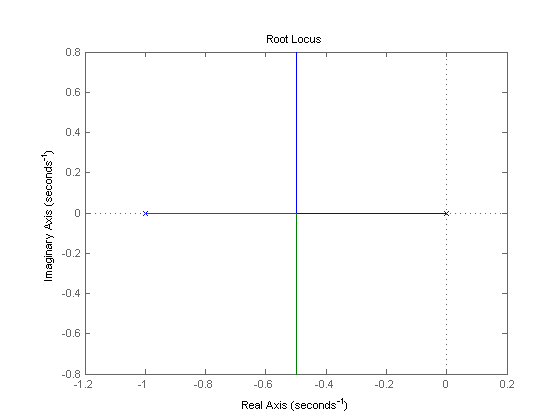
\includegraphics[scale=0.6]{./pictures/experimento1_LGR_original.png}
			\caption{LGR origial do experimento 1}
			\label{fig:experimento1_LGR_original}
		\end{figure}
		\begin{figure}[h!]
			\centering
			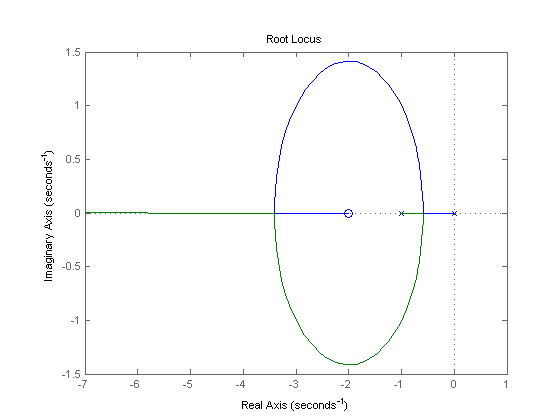
\includegraphics[scale=0.6]{./pictures/experimento1_LGR_zero.png}
			\caption{LGR com adi��o de umz zero do experimento 1}
			\label{fig:experimento1_LGR_zero}
		\end{figure}
		\begin{figure}[h!]
			\centering
			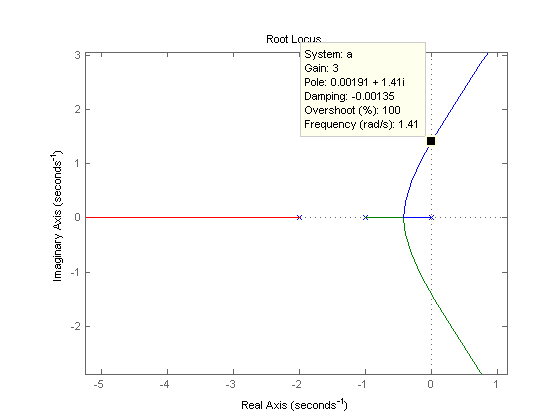
\includegraphics[scale=0.6]{./pictures/experimento1_LGR_polo.png}
			\caption{LGR com adi��o de um p�lo do experimento 1}
			\label{fig:experimento1_LGR_polo}
		\end{figure}
	

\chapter{Experimento 2}

\chapter{Experimento 3}

\chapter{Experimento 4}
		
\end{document}
